\documentclass[journal]{vgtc}                % final (journal style)
%\documentclass[review,journal]{vgtc}         % review (journal style)
%\documentclass[widereview]{vgtc}             % wide-spaced review
%\documentclass[preprint,journal]{vgtc}       % preprint (journal style)

%% Uncomment one of the lines above depending on where your paper is
%% in the conference process. ``review'' and ``widereview'' are for review
%% submission, ``preprint'' is for pre-publication, and the final version
%% doesn't use a specific qualifier.

%% Please use one of the ``review'' options in combination with the
%% assigned online id (see below) ONLY if your paper uses a double blind
%% review process. Some conferences, like IEEE Vis and InfoVis, have NOT
%% in the past.

%% Please note that the use of figures other than the optional teaser is not permitted on the first page
%% of the journal version.  Figures should begin on the second page and be
%% in CMYK or Grey scale format, otherwise, colour shifting may occur
%% during the printing process.  Papers submitted with figures other than the optional teaser on the
%% first page will be refused. Also, the teaser figure should only have the
%% width of the abstract as the template enforces it.

%% These few lines make a distinction between latex and pdflatex calls and they
%% bring in essential packages for graphics and font handling.
%% Note that due to the \DeclareGraphicsExtensions{} call it is no longer necessary
%% to provide the the path and extension of a graphics file:
%% 
\includegraphics{diamondrule} is completely sufficient.
%%
\ifpdf%                                % if we use pdflatex
  \pdfoutput=1\relax                   % create PDFs from pdfLaTeX
  \pdfcompresslevel=9                  % PDF Compression
  \pdfoptionpdfminorversion=7          % create PDF 1.7
  \ExecuteOptions{pdftex}
  \usepackage{graphicx}                % allow us to embed graphics files
  \DeclareGraphicsExtensions{.pdf,.png,.jpg,.jpeg} % for pdflatex we expect .pdf, .png, or .jpg files
\else%                                 % else we use pure latex
  \ExecuteOptions{dvips}
  \usepackage{graphicx}                % allow us to embed graphics files
  \DeclareGraphicsExtensions{.eps}     % for pure latex we expect eps files
\fi%

%% it is recomended to use ``\autoref{sec:bla}'' instead of ``Fig.~\ref{sec:bla}''
\graphicspath{{figures/}{pictures/}{images/}{./}} % where to search for the images

\usepackage{microtype}                 % use micro-typography (slightly more compact, better to read)
\PassOptionsToPackage{warn}{textcomp}  % to address font issues with \textrightarrow
\usepackage{textcomp}                  % use better special symbols
\usepackage{mathptmx}                  % use matching math font
\usepackage{times}                     % we use Times as the main font
\renewcommand*\ttdefault{txtt}         % a nicer typewriter font
\usepackage{cite}                      % needed to automatically sort the references
\usepackage{tabu}                      % only used for the table example
\usepackage{booktabs}                  % only used for the table example
\usepackage{multirow}
\usepackage{enumitem}
%% We encourage the use of mathptmx for consistent usage of times font
%% throughout the proceedings. However, if you encounter conflicts
%% with other math-related packages, you may want to disable it.

%% In preprint mode you may define your own headline.
%\preprinttext{To appear in IEEE Transactions on Visualization and Computer Graphics.}

%% If you are submitting a paper to a conference for review with a double
%% blind reviewing process, please replace the value ``0'' below with your
%% OnlineID. Otherwise, you may safely leave it at ``0''.
\onlineid{0}

%% declare the category of your paper, only shown in review mode
\vgtccategory{Research}
%% please declare the paper type of your paper to help reviewers, only shown in review mode
%% choices:
%% * algorithm/technique
%% * application/design study
%% * evaluation
%% * system
%% * theory/model
\vgtcpapertype{please specify}

%% Paper title.
\title{Crowd-powered Semantic Ineraction for Text Analytics}

%% This is how authors are specified in the journal style

%% indicate IEEE Member or Student Member in form indicated below
\author{Yali Bian, Tianyi Li, Ji Wang, Kurt Luther, Chris North}
\authorfooter{
%% insert punctuation at end of each item
\item
 Yali Bian, Kurt Luther, Chris North are with Virginia Tech. E-mail: [yali, north]@vt.eud.
}

%other entries to be set up for journal
\shortauthortitle{Biv \MakeLowercase{\textit{et al.}}: Global Illumination for Fun and Profit}
%\shortauthortitle{Firstauthor \MakeLowercase{\textit{et al.}}: Paper Title}

%% Abstract section.
\abstract{
Visual analytics could help users explore and gain insight from dataset through interactive visualization and underlying data analytics models.
However,  understanding of large text dataset is still challenging in many domains.
For example, an intelligence analyst might need to find a coordinated terrorist assault in three US cities from one hundred of documents in a limited time.
Existing visual analytics techniques only assist with low-level tasks, such as finding related documents based on shared entities, which still require significant effort on the part of users.

To support the high-level sensemaking process in visual analytics, we present the framework of crowd-powered semantic interaction, where semantic interactions \textit{[citations]} can be used assign micro-tasks to crowds, and forges the crowds feedbacks for final decisions of expert users.
This model could help users to steer crowd-workers to carry out sensemaking tasks implicitly even they are novice on crowdsourcing.
The completed crowds feedbacks would be used to update the visualization appropriately that foster the related foraging and synthesis parts for users.

To explain this model, we introduce CrowdSPIRE, a visual text analytics concept proof prototype that converts user interactions on documents into micro-tasks called "Connect the Dots".
For example, the user drags two texts together, which triggers the assignment of certain sensemaking tasks to crowdworkers automatically,  in parallel with the expert’s own investigation.
When the tasks finished, crowds feedbacks could be used to update current visualization appropriately without distracting users' attention from their process.
}

%% Keywords that describe your work. Will show as 'Index Terms' in journal
%% please capitalize first letter and insert punctuation after last keyword
\keywords{Visual analytics, Semantic Interaction, Crowdsourcing, Sensemaking, Crowd-powered Interface. }

\CCScatlist{ % not used in journal version
 \CCScat{K.6.1}{Management of Computing and Information Systems}%
{Project and People Management}{Life Cycle};
 \CCScat{K.7.m}{The Computing Profession}{Miscellaneous}{Ethics}
}

%% Uncomment below to include a teaser figure.
\teaser{
  \centering
  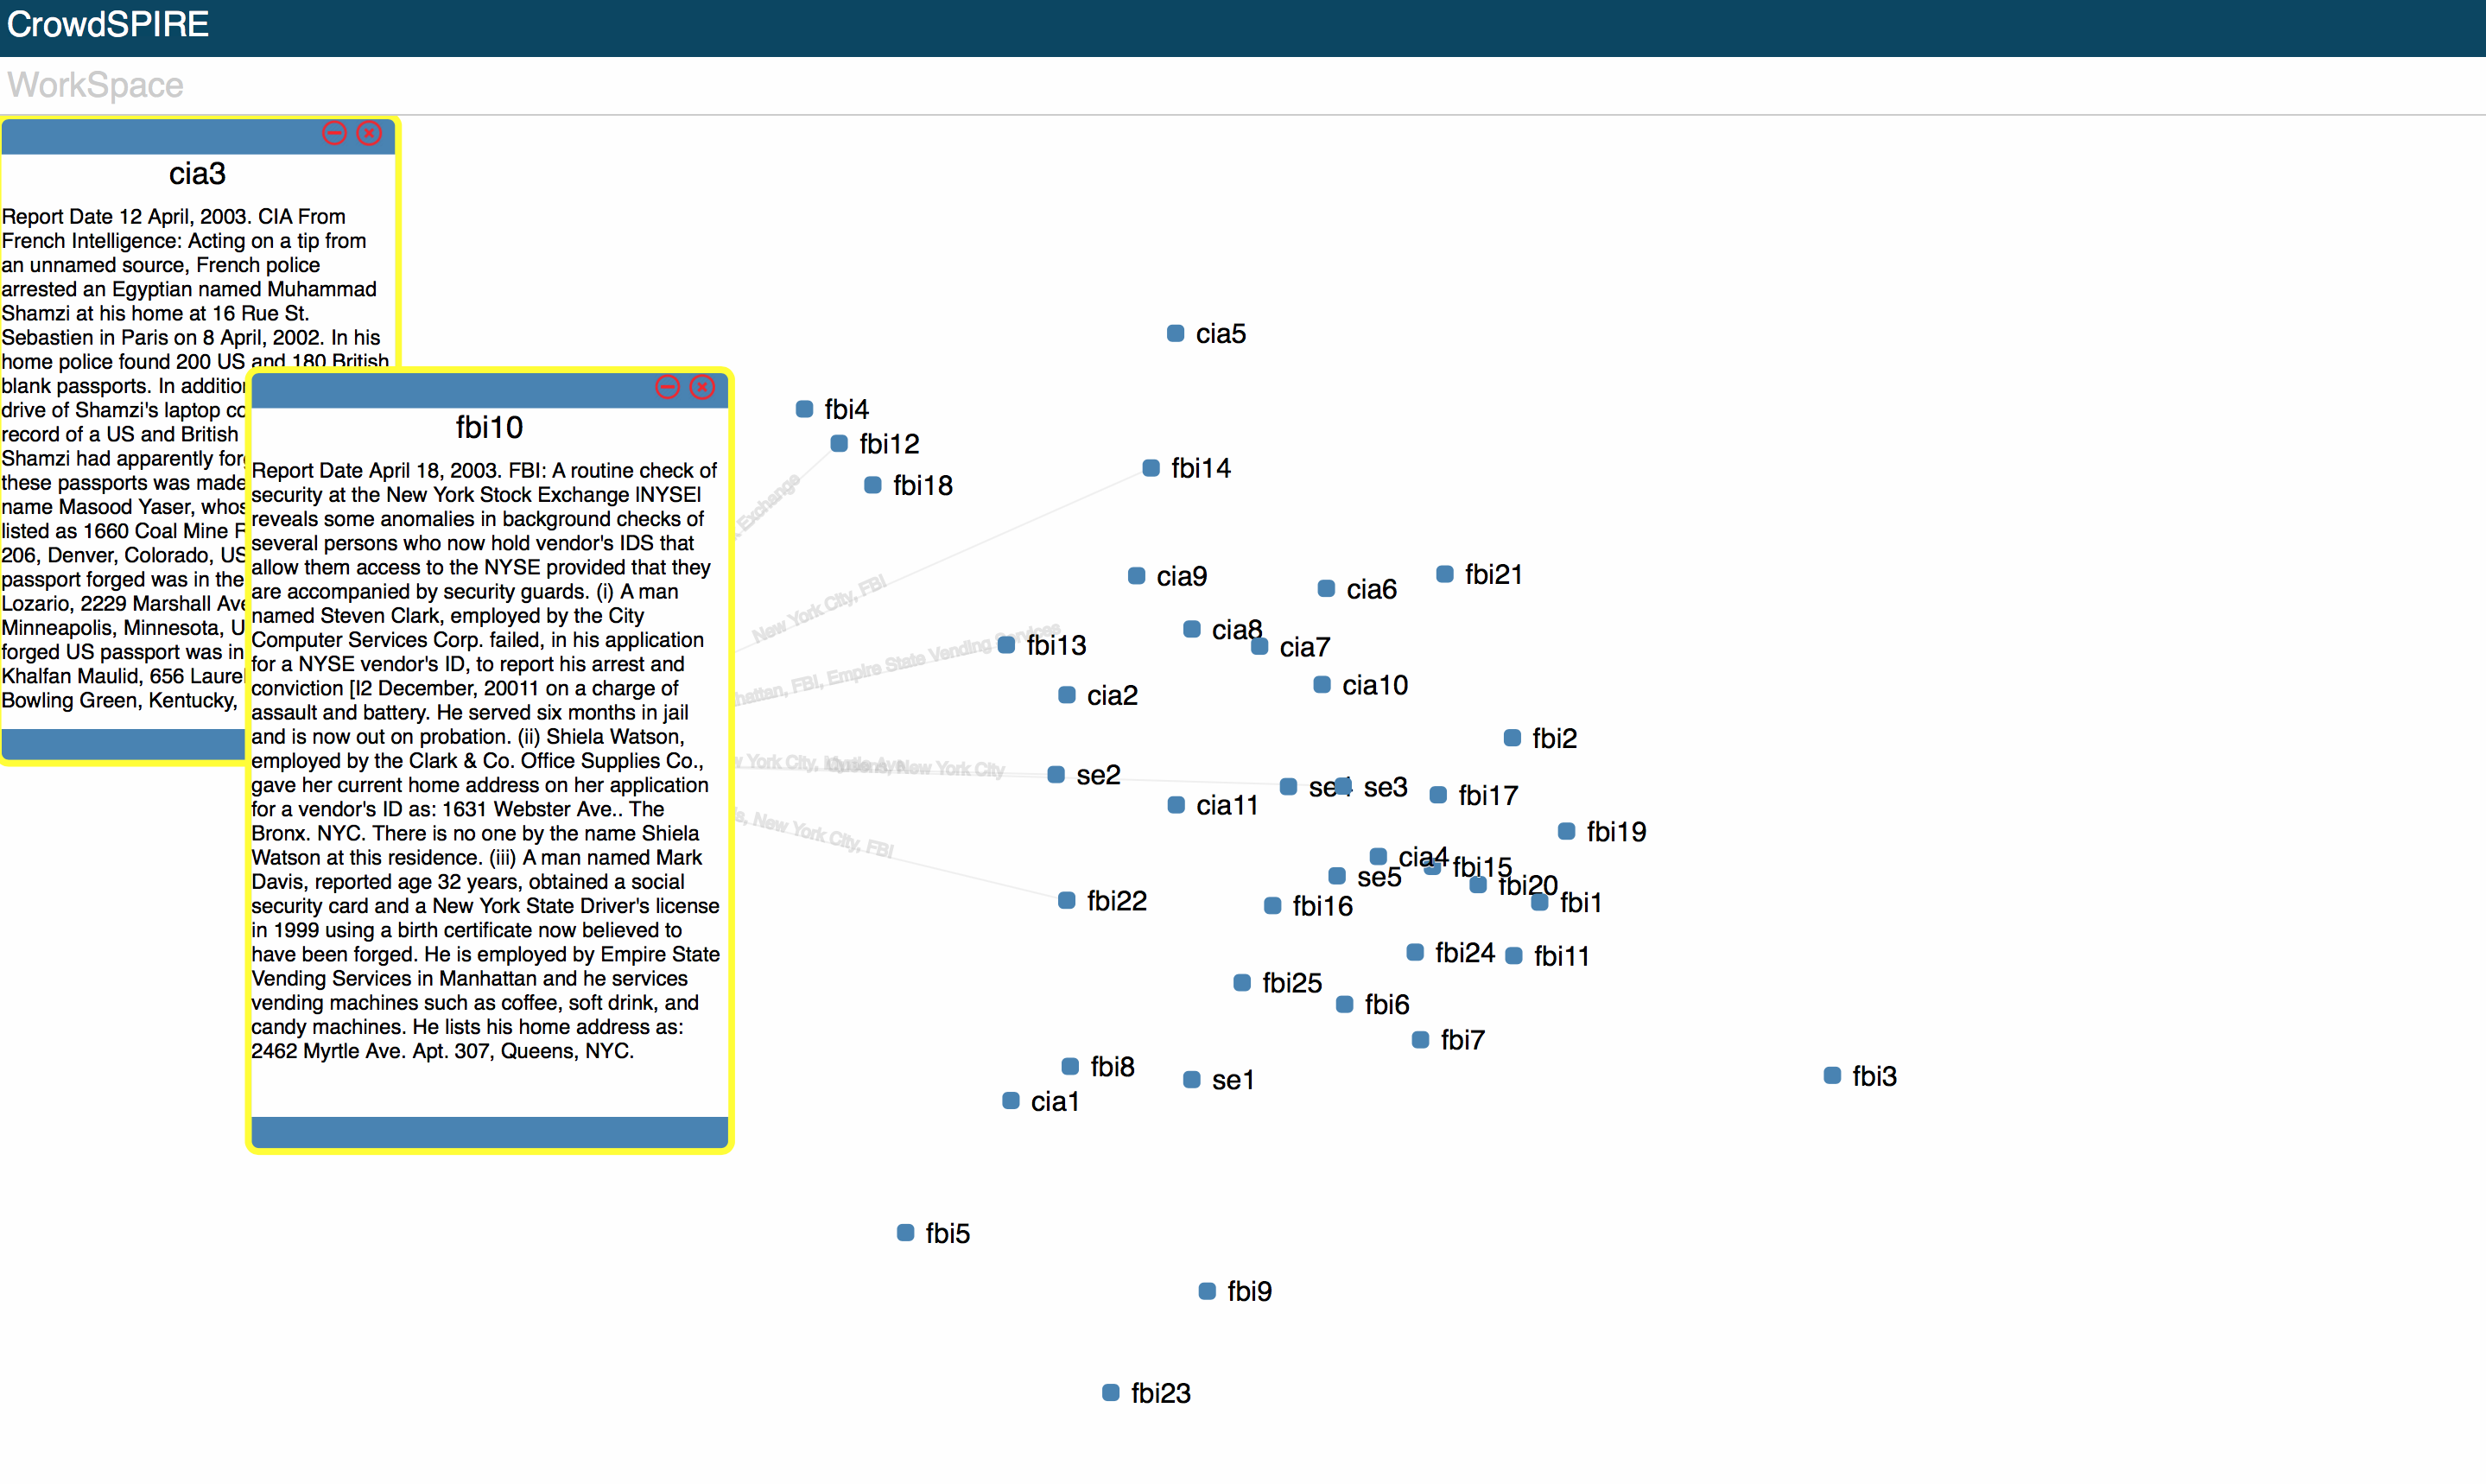
\includegraphics[width=\linewidth]{Overview}
  \caption{Crowd-powered Senmantic Interaction for Text Analytics}
	\label{fig:Overview}
}

%% Uncomment below to disable the manuscript note
%\renewcommand{\manuscriptnotetxt}{}

%% Copyright space is enabled by default as required by guidelines.
%% It is disabled by the 'review' option or via the following command:
% \nocopyrightspace
\vgtcinsertpkg

%%%%%%%%%%%%%%%%%%%%%%%%%%%%%%%%%%%%%%%%%%%%%%%%%%%%%%%%%%%%%%%%
%%%%%%%%%%%%%%%%%%%%%% START OF THE PAPER %%%%%%%%%%%%%%%%%%%%%%
%%%%%%%%%%%%%%%%%%%%%%%%%%%%%%%%%%%%%%%%%%%%%%%%%%%%%%%%%%%%%%%%%

\begin{document}

%%%%%%%%%%%%%%%%%%%%%%%%%%%%%%%%%%%%%%%%%%%%%
%	Introduction
%%%%%%%%%%%%%%%%%%%%%%%%%%%%%%%%%%%%%%%%%%%%%
\firstsection{Introduction}
\maketitle
%% \section{Introduction}
Understanding large amount of unstructured text is emering today. If we can find ways to make sense of them, the possibilities for learning more about ourselves and how to improve the world we live in are almost boundless. 
For example, detecting and preventing a terrorist attack based on intelligence reports. Responding to the challenging, there emerged the field of visual analytics\cite{Thomas2005} that combines the powerful approaches--information visualization\cite{card1999readings} and data mining\cite{berry1997data} --to create a new class of sensemaking tools\cite{Pirolli2005} enabling new kinds of exploration and insights. (Exemple)

However, it remains time-consuming and onerous, and existing support tools still have a long way to go. Machine learning techniques could help find clusters and summarize documents efficiently, but currently, they cannot generate questions, hypotheses, or conclusions based on data that are more subtle than what an algorithm has been programmed to recognize. What's more, visualization tools amplify the cognitive abilities of their users, but many users could only access to low-level information on documents, which requiring significant effort on the part of users to get the deep insight of data with all kinds of external knowledge. For example, analysts cannot find the relationship between AMTRAK \#19 with a terrist attack if they don't consult the AMTRAK schedules on the Internet to see that Train \#19 is in fact called "The Crescent."


% Corresponding model updates are performed to steer the model based on the user’s reasoning.
% Why Crowdsoucing, why crowdsoucing hard to use
Crowdsourcing presents new opportunities to deal with this issue by augmenting the cognitive work of individual analysts, providing more insightful analysis than automated approaches and scaling better than traditional work. Crowdsourcing was originally used for simple, independent tasks that leverage innate human abilities like transcribing text\cite{causer2012transcription}, identifying images\cite{gupta2013faking}, and categorizing or labeling items\cite{bragg2013crowdsourcing}. Recently, researchers have begun to investigate how crowdsourcing can be applied to complex sensemaking tasks, like creating a taxonomy of items\cite{Chilton2013} planning a vacation\cite{Zhang2012} or writing a news article\cite{kittur2011crowdforge}. These efforts show promise for how crowds might assist an individual analyst with a difficult sensemaking problem.

Though crowdsourcing is a powerful method to enhance users sensemaking process, the integration of crowdsourcing into visual analytics could be tough work. Analysts who are non-expert in crowdsourcing might have a hard time to design and assign tasks to crowds. Even they are experts on human computation; they still have to put their time and energy in designing appropriate HITs and putting it to a crowdsourcing platform, which will distract analysts from their current investigation. [More details?]

% Steer crowdsourcing implicitly.
Semantic interaction\cite{Endert2014} has been approved to a be a good way to help users focus on their cognition of interesting elements on visualization, at the same time steering underlying models implicitly\cite{Endert2012}. Through basic interactions like dragging documents together, highlight important sentences, analysts could steer computational analytical models implicitly, instead of mastering the model first and changing the low-level input parameters of algorithms directly. Semantic interaction provides a bridge between analysts who are non-expert on machine learning algorithms and underlying models.

With semantic interaction, an expert analyst could guide the machine learning algorithms by directly manipulating the visualization layout. Our vision is that the expert interactions will also guide crowdsourcing micro-tasks to do more sensemaking works that machine learning algorithms not good at. We propose the crowd-powered semantic interaction model by coupling visual analytics with crowdsourcing through semantic interaction, and therefore, coupling analysts not only with the ability to parse huge quantities of documents but also the power to make sense of complex tasks effectively.

Designing visual analytics systems with crowdsourcing involves new challenges that we should take into consideration. Visual analytics system should map interactions to appropriate relevant sensemaking tasks semantically. For example, it is not a good idea to map interaction of dragging two documents aways from each other to micro-tasks that find their similarities. Also, coordinating and aggregating different kinds of tasks to effectively contribute to sensemaking visual feedback is another problem. Since different sub-tasks could have different granularity, information context, correctness, and efficiency.

To address such challenges, we present the crowd-powered semantic interactions to support the combination of visual analytics with human computations. Our key contributions in this paper are as follows:

(1) We propose the crowd-powered semantic interaction model that improve users' sensemaking process through crowdsourcing and formalize this model in the form of an updated visualization pipeline enhanced with crowdsourcing.

(2) We formalize the mapping from interaction to micro-tasks as sensemaking allocation strategies based on the user’s reasoning.

(3) We classify current existing sensemaking crowdsourcing tasks for text analytics based on their granularity and efficiency and explore the solutions to integrate them into real-time visual analytics system.

(4) To demonstrate crowd-powered semantic interaction, we present CrowdSPIRE, a visual analytics prototype based on ForceSPIRE. We present a usage scenario to demonstrate how crowd-powered semantic interactions to be used to help users' complex sensemaking tasks.



%%%%%%%%%%%%%%%%%%%%%%%%%%%%%%%%%%%%%%%%%%%%%
%	Related Work
%%%%%%%%%%%%%%%%%%%%%%%%%%%%%%%%%%%%%%%%%%%%%
\section{Related Work}

The key idea of crowd-powered semantic interaction is enhancing visual analytics's ability to leverage users' cognition for complex sensemaking tasks with crowdsourcing through semantic interaction. Two key aspects are involved in this model: semantic interaction for visual analytics, crowdsourcing sensemaking tasks and crowd-powered system\cite{Bernstein2012}.

\subsection{Semantic Interaction}


% What is semantic interaction

Visual analytics\cite{Thomas2005} combines the powerful approaches information visualization, and data mining together that creates a new class of sensemaking tools enabling new kinds of exploration and insights. Usually, visual analytics systems provide visualized parameters such as controller bars\cite{Jeong:2009gc} to help users directly steer lower-level computational models. For that kind of applications, the analyst needs to an expert in the underlying model based on their input parameters.

Semantic interaction makes visual analytic systems available for people who are not familiar with underlying mining method. Instead of providing interactions for controlling low-level input parameters of the algorithms, visual analytics with semantic interactions provides high-level interactions, which could be recast into low-level inputs through machine learning algorithms that attempt to recognize the reasoning process. \autoref{fig:SemanticInteraction} illustrates this the difference between basic visual analytics system and visual analytics system with semantic interaction, where the spatialization is treated as a medium through which the user can perceive information and gain insight, as well as interact and perform his analysis.

Semantic interaction successfully recognized analysts’ reasoning processes and relieved users from the need to organize many supporting documents or read many irrelevant documents \cite{Endert:2012wq}. We now recognize the opportunity to apply semantic interaction techniques to enable analysts to not only direct computational algorithms but also to manage a large force of crowd workers. Also, since semantic interaction recognizes opportunities for supporting subtasks and relevant information, it could also be used to narrow down context that the micro-tasks needed should assigned to crowd workers.

\begin{figure}[tb]
 \centering % avoid the use of \begin{center}...\end{center} and use \centering instead (more compact)
 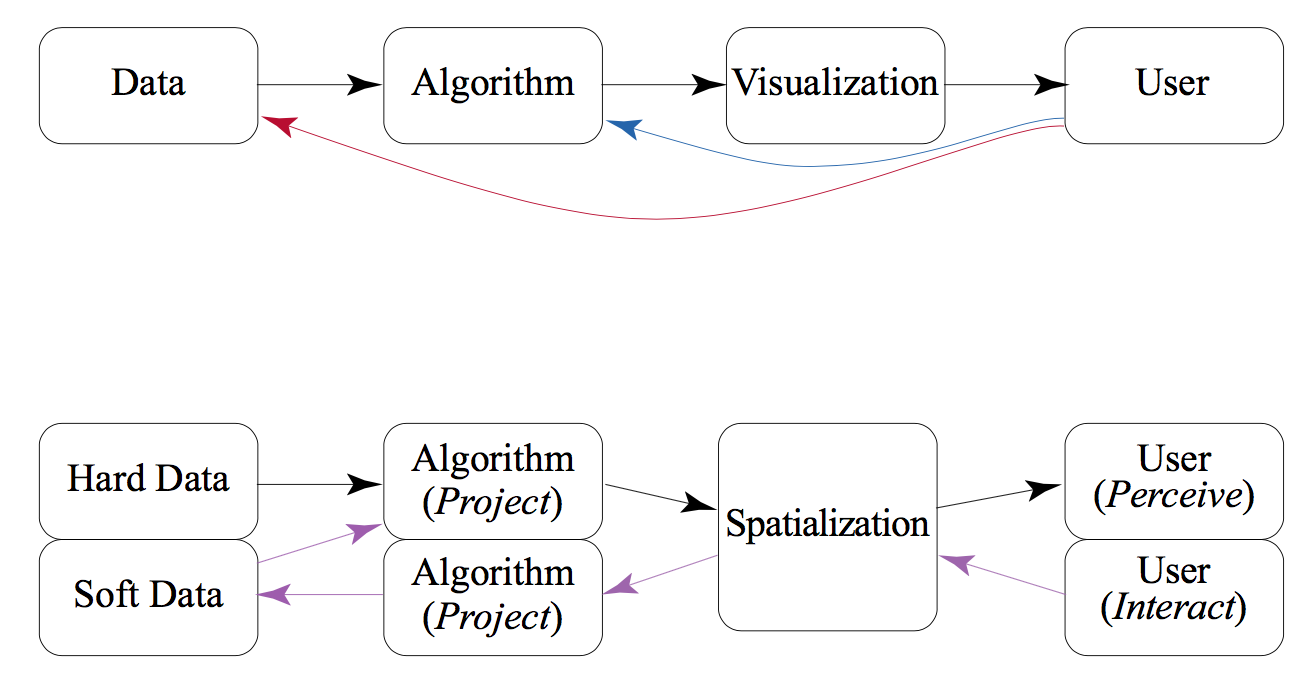
\includegraphics[width=\columnwidth]{SemanticInteraction}
 \caption{ (top) The basic version of the “visualization pipeline.” Interaction can be performed di- rectly on the algorithm (blue arrow) or the data (red arrow). (bottom) Our modified version of the pipeline for semantic interaction, where the user interacts within the spatial metaphor (purple arrow). The image is from \cite{Endert:2016co}}

 \label{fig:SemanticInteraction}
\end{figure}


\subsection{Crowdsourcing}

Crowdsourcing\cite{Law:2011cq} is a new and emerging research field that could help accomplish complex tasks with which computers typically struggle, such as image labeling, language translation\cite{zaidan2011crowdsourcing}.
Nowadays, online crowdsourcing marketplaces like Amazon Mechanical Turk\cite{MTurk} where distributed groups of people complete small amounts of work (micro-tasks) for money make the use of human intelligence to perform tasks much available. Crowdsourcing has even been embedded in software back-ends and user interfaces to provides complex services, like, answering to visual questions\cite{Bigham:2010cj}.


% \begin{figure}[tb]
\begin{figure*}[!htbp]
 \centering % avoid the use of \begin{center}...\end{center} and use \centering instead (more compact)
%  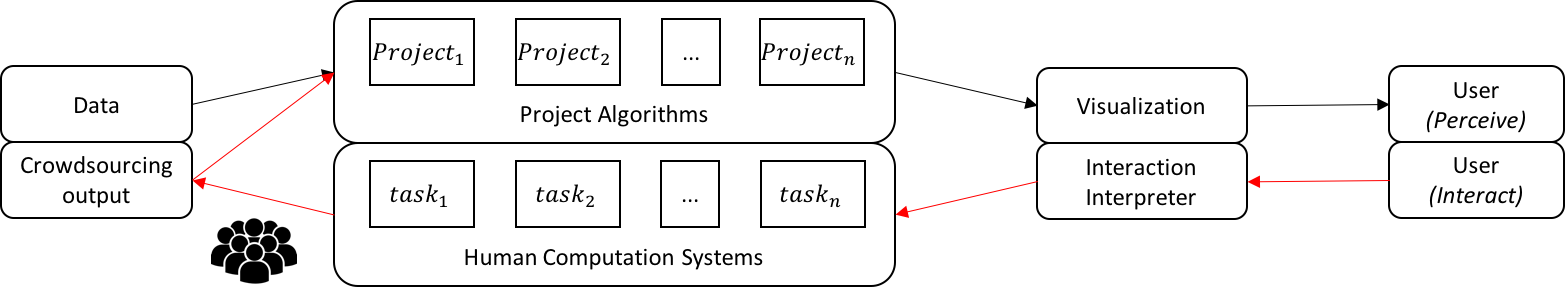
\includegraphics[width=\columnwidth]{Pipeline}
  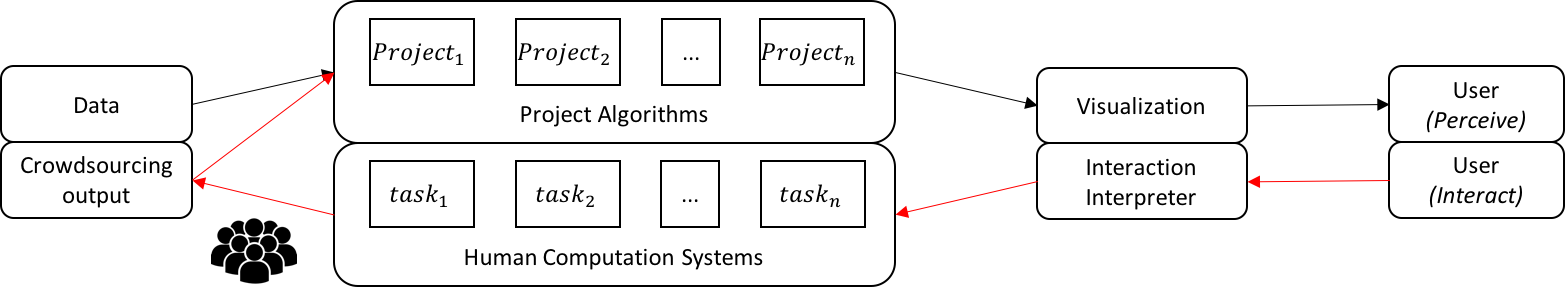
\includegraphics[width=\textwidth]{Pipeline}
 \caption{crowdsourcing based semantic interaction visualization pipeline.
 Once the user perceives the visualization, they can choose to interact in it.
 This interaction feedback is interpreted as requests to the human computation system, which could assign several micro-tasks to crowds.
 The project algorithms could update visualization based on crowdsourcing outputs through their types, along with original data.
	 }
 \label{fig:Pipeline}
\end{figure*}

\subsubsection{Crowdsourced sensemaking tasks}
Current research on crowdsourcing has changed from simple, independent tasks like images labeling\cite{welinder2010online} to more complex and creative tasks, like planning a vacation\cite{Zhang2012}. What's more, researchers start to investigate how to apply crowdsourcing to complex sensemaking tasks, like creating a taxonomy of items or performing a bottom-up analysis of a large corpus of qualitative data, often with algorithms or workflows that decompose large tasks into smaller ones that can be completed in parallel.

Sensemaking\cite{Pirolli2005} is a difficult process that involves tasks: finding relevant information, relating heterogenous concepts, forming hypotheses, justifying arguments, reconciling conflicting or missing data, making inferences and complex reasoning\cite{Thomas2005}. There exist lots of crowdsourcing research explorations differ in their emphasis on different kinds of sensemaking tasks:  Crowdnection\cite{Wang:2016cb}, uses crowdsourcing to help connect high-level concepts through documents or raw texts. Cascade\cite{Chilton2013} produces crowdsourced taxonomies of hierarchical data sets by letting crowd works generate and later select, multiple categories per item. Frenzy\cite{Chilton2014} is a collaborative session organizer that classify papers into sessions based on their metadata. Crowdlines\cite{Luther2015} explores how crowd works can synthesize information from diverse sources gathered online to produce a useful overview.

Visual analytics systems with crowd-powered semantic interaction could make full use of those great crowdsourcing research explorations on sensemaking as the underlying models that help mining complex documents and provides those crowd-processed information to users.

\subsubsection{Crowd-powered System}
With crowdsourcing in the computation to be universal, embedding human computation into applications to help carry out complex tasks that automatic computation is not skilled could be a good solution. And those kinds of applications with both automatic and human computation are called crowd-powered system.

However, crowdsourcing tasks that are usually time-consuming, making it difficult to incorporate and take advantage of crowds in real word applications. Lots of advanced crowdsourcing algorithms have been proposed to make crowd-powered systems easier to implement in real time.

VizWiz\cite{Bigham2010} provides a nearly real-time application to answer to visual questions by predicting and posting possible jobs to several crowd workers before users request directly. Soylent\cite{Bernstein2010} is a crowd-powered word processor that divide writing tasks into small pieces that could be processed by crowd-workers parallely.

Adrenaline \cite{Bernstein2011} is a camera with crowsourcing where crowds could help pick the bset monent photo from a video. It could repsonse to user's input within seconds based on the recruiting strategies to use synchronous crowd workers and dynamically adapt tasks. Chorus\cite{Lasecki2013} is a conversational assistant that enables real-time interactions based on collaborative reasoning, dynamic scoring system and curated memory system.

Using these techniques, we could prototype out interactive crowd-powered visual analytics system that can provider users interactions feedbacks in real time and extends them to complex sensemaking tasks where crowds are directed by mechanisms other than explicit user requests.

%%%%%%%%%%%%%%%%%%%%%%%%%%%%%%%%%%%%%%%%%%%%%
%	Crowd-Powered Semantic Interaction
%%%%%%%%%%%%%%%%%%%%%%%%%%%%%%%%%%%%%%%%%%%%%
\section{Pipeline}


\begin{table*}[t]
  \caption{Forms of crowd-powered semantic interaction. Each interaction corresponds to reasoning of users within the analytic process. Corresponding model updates are performed to steer the model. Corresponding allocation strtegy used to assign crowd tasks.}
  \label{tab:SensemakingTasks}
  \centering
  \begin{tabular}{| m{2.5cm} | m{4.5cm} | m{4.5cm} | m{4.5cm} |}
%  \begin{tabular}{| p{2.5cm} | p{4.5cm} | p{4.5cm} | p{4.5cm} |}
  \hline
   Semantic \newline Interaction & Associate Analytic Reasoning & Model Updates & Sensemaking Task \\ \hline

Document \newline Movement  & \begin{itemize} [leftmargin=.1in]
                                \item Similarity/Dissimilarity
                                \item Create spatial construct (e.g. cluster, timeline, list, etc.)
                                \item Test hypothesis, see how document \lq fits\rq \ in region
                              \end{itemize}
                            &
                               \begin{itemize}  [leftmargin=.1in]
                                 \item Similarity/Dissimilatiry b/w documents
                                 \item Up-weight shared entities, down-weight others
                               \end{itemize}
                            &  \begin{itemize} [leftmargin=.1in]
                                 \item Rank or group documents based on similarity/dissimilarity b/w docuemnts.
                                 \item Describe why documents are similiar/dissimilar to each other semantically.
                               \end{itemize} \\ \hline

Text Highlighting & \begin{itemize} [leftmargin=.1in]
                                 \item Mark importance of phrase (collection of entities)
                                 \item Augment visual appearance of document for reference
                               \end{itemize}
                  & \begin{itemize} [leftmargin=.1in]
                                 \item Up-weight highlighted entities
                               \end{itemize}
                  & \begin{itemize}[leftmargin=.1in]
                                 \item  Find more related entities that has the same meaning semantically.
                                 \item  Find more related documents that contain the same concept of highlighted entities
                               \end{itemize} \\ \hline

Pinning Document to Location & \begin{itemize} [leftmargin=.1in]
                                    \item Give semantic meaning to space/layout
                               \end{itemize}
                             &  \begin{itemize} [leftmargin=.1in]
                                    \item Layout constraint of specific document
                               \end{itemize}
                             & \begin{itemize} [leftmargin=.1in]
                                    \item Cluster or rank documents based on distances between pinned documents
                               \end{itemize} \\ \hline

Annotation, “Sticky Note” & \begin{itemize} [leftmargin=.1in]
                                    \item Put semantic information in workspace, within document context
                               \end{itemize}
                          & \begin{itemize} [leftmargin=.1in]
                                    \item Up-weight entities in note
                                    \item Append tities to document and model
                            \end{itemize}
                          & \begin{itemize} [leftmargin=.1in]
                                    \item Interpret entities in note, and find more related entities
                                    \item Find more related documents based on notes.
                            \end{itemize} \\ \hline


Level of Visual \newline Detail (Document vs. Icon) & \begin{itemize} [leftmargin=.1in]
                                                \item Change ease of visually referencing information (e.g., full detail = more important = easy to reference)
                                             \end{itemize}
                                           &  \begin{itemize} [leftmargin=.1in]
                                                \item (Full Document): “heavier node,” increase node’s friction
                                                \item (Icon): “lighter node,” less friction
                                             \end{itemize}
                                           & \begin{itemize} [leftmargin=.1in]
                                                \item (Full Document): Rank and group documents related to opened document.
                                                \item (Icon): Remove documents related to the closed document.
                                             \end{itemize} \\ \hline

Search Terms & \begin{itemize}[leftmargin=.1in]
                   \item Expressive search for entity
               \end{itemize}
             & \begin{itemize}[leftmargin=.1in]
                    \item Up-weight entities contained in search
                    \item Add entities to model
               \end{itemize}
             & \begin{itemize}[leftmargin=.1in]
                    \item Inteprete serached terms and find more related entities semantically.
                    \item Find the most related documents that contain searched terms semantically
               \end{itemize} \\ \hline

\end{tabular}
\end{table*}

To leverage users from complex sensemaking tasks, we propose the crowd-powered semantic interaction. As shown on \autoref{fig:Pipeline}, visual analytics systems with crowd-powered semantic interaction could detect users' current sensemaking tasks based on their interactions; then complex tasks could be decomposed into sub-tasks and assigned to crowd workers; finally, recombine sub-task outputs and convey it via visual feedback to analysts.

We present an updated visual text analytics pipeline to reflect our crowd-powered semantic interaction model.  At first, analysts will get an overview of original data based on underlying map and layout visualization algorithm. The user then could perceive data through their corresponding visual elements and explore interesting documents through searching terms and make sense of texts through interactions: such as text highlighting and documents movement.


Though the model of semantic interaction, interactions could be interpreted to user's current analytical reasoning with specific contexts. To be more specific, based on the controlled visual object, current visualization contexts, and interaction, we could determine user's sensemaking task in details. Then the specified sensemaking task could be projected to the crowdsourcing task that could be easily implemented. Not all sensemaking tasks will be directly projected to crowdsourcing HITs because the sensemaking task is too complex. For this situation, tasks should be decomposed into sub-tasks. For example, the sensemaking task corresponds to current interaction is compare two documents and find related documents based on two documents' similarities. We need at first, divide this task into finds connections between two documents, and finding relevant documents based on connections. When tasks finished nearly real-time, the crowdsourcing outputs combined with original data could again project to current visualization based on map and layout algorithms.

For example, an expert working in intelligence analysis has lots of reports to analyze in our visual analytics system with crowd-powered semantic interaction. The expert begins sifting through and grouping related documents. He puts three documents about "New York Stock Exchange" and "C-4" together to form a cluster. Meanwhile, the system creates sensemaking task of finding related documents. The system recruits crowd workers to suggest potentially documents that belong to the groups. Then the visualization updated based on the crowdsourcing results: there are three more documents emerged on the cluster: even those documents don't contain the keyword "New York Stock Exchange" or "C-4", but they do contain "NYSE" and "Explosive." After analyse this cluster, the expert find enough evidence that a terrist group plan to bomb out the NYSE building.

Possible extension of this pipeline is combining automatic computation together with human computation to support users with sensemaking and computation power. Moreover, human computation and automatic computation could also provide modifications for each other. For example, system could dynamically control micro-tasks, based on removing irrelevant documents through data mining methods.

Two key techniques are involved in crowd-powered interaction: mapping interactions to sensemaking tasks based on task allocation strategy and updating visualization model based on crowds output. In the following two subsections, we discuss them in detail and explain how these techniques to improve users' sensemaking loop.


\section{Crowd-powered Semantic Interactions}




The most important step on crowd-powered semantic interactions is mapping interactions to crowdsourcing tasks. It is essential that crowdsourcing tasks could determine why interaction occurred, and the completed outputs could provide positive help to analysts. To make sure visual analytics system could assign crowdsourcing tasks accurately and rationally, we represent the task allocation strategy (See \autoref{tab:SensemakingTasks}) based on previous findings\cite{andrews2010space} that user interactions can be associated with particular forms of analytical reasoning.


For original semantic interaction, the system determines the analytical reasoning associated with the interactions and updates the model accordingly\cite{Endert2012V}. Analogously, systems with crowd-powered semantic interactions  determines the analytical reasoning associated with interactions and assign tasks to crowds accordingly.

Current semantic interactions for text analytics mainly based on sptatializations[], a good medium helps users organize and maintain their hypotheses and insights. What's more,   spatializations of document sets exist that allow users to place “points of interest” directly into the spatial layout. Thus, assigned sensemaking tasks are primarily used to update document spatialization. So the output of sensemaking tasks for text analytics should be easily used to update document spatializations accurately. If we could use crowd workers to help update the document layout based on user's organizational schema, user could finish their sensemaking quickly. For different interaction, we could design and assign sensemaking HITs to crowd workers based on current interaction contexts and associate analytic reasoning. We describe crowd-powered interactions for text analytics based on original semantic interactions[] as shown on \autoref{tab:SensemakingTasks}: document movement, text highlighting, pinning document to location, annotation sticky note, change level of visual detail and search terms. In the rest part of this subsection, we will talk how those interactions could be used to direct related tasks in details, and compare them with corresponding algorithm moedels.

\subsection{Interactions to sensemaking tasks}

For visual analytics, we define three kinds of sensemaking tasks to present interactions in three levels.

\textbf{Document movement} is the most common used interaction that lets users drag documents to different positions which allow users to explore the relationship of that document in comparison to the remaining documents.  When dragging a document close to or away from one or a group of documents, crowdsourcing tasks of showing the dragged documents and related documents to crowd-workers and require them to rank their relationship again.

\textbf{Text highlighting} shows selected text might contains very imporatant clues, crowdsourcing could help synthsis this clues, such as find high level concepts or related entities on current document or find more related documents about selected texts.

\textbf{Pinning document to location}: Pinning documents to different locations gives semantic meaning to that place, crowdsourcing tasks should help fill out those places through tasks:  find documents similar to only one of the pinned document which should locate close to this document, or find documents related to all of the pinned documents, that should locate near both of the pinned documents.

\textbf{Annotation, sticky note}: Annotating a documet trigger two kind of sensemaking tasks: analyse inputted notes based on selected document, with high-level concept and entities; find most relavant documents based on nodes, and concepts.

\textbf{Level of visual detail}: Minimizing a document could trigger crowdsourcing task that finding more dissimilar documents. Open a document could trigger crowdsourcing task of finding more similar documents related to the opened document.

\textbf{Search terms}: Searching for a term meaning finding more related documents that contain the term semantically. During this interaction, underlying crowdsourcing task is mainly about annotate inputted terms with high level concepts or entities, then let crowd workers find the most related documents.



%%%%%%%%%%%%%%%%%%%%%%%%%%%%%%%%%%%%%%%%%%%%%
% Sensemaking tasks to crowdsourcing tasks
\subsection{Crowdsourcing Task Choices for Sensemaking Task}

Several visual representations for graph layouts and interaction tech- niques have been discussed in [84], many of which can potentially be applied to present and explore Entity-LR and Group-LR. Entity-LR are easy for humans to interpret.

We define sensemaking tasks based on users' intentions that visual analytics systems could provide help on.  For systems with crowd-powered semantic interaction, sensemaking tasks could be carried out through crowdsourcingt tasks. For each kind of sensemaking task, there exiting several kinds of crowdsourcing taks help solve those sensemaking tasks.

Two ways of find the layout of crowdsourcing ways.

Since our sensemaking tasks could be mapped to distance between documents. We could calculate the distance between documents in different levels. Document contents level and document level. We calculate the document connections to calculate their similarity or based on pairwise ranking aggregation. Instead of calculate their relationships through connections. We could also rank their similarity between two documents.

For the first kind of solution, we call them 'Connect the Dots' and the second one 'Pairwise ranking aggregation'.

\subsubsection{Connect the Dots}

Researchers have explored the value of using
crowdsourcing, either alone or combined with
automated approaches, to synthesize information with
diverse or unknown schemas. One fruitful approach has been to blend crowdsourcing with ML algorithms. Partial clustering [19,40] and crowd kernel [35] are two such examples, but their application domain limited to imagery, and they focus on low context merges between pairs or triplets of items.


CONNECTING DOCUMENT PAIRS through
The connection types identified were entity, conceptual, temporal, speculative, and domain knowledge
High-level connections involved users relating information gleaned from the data with their own cognitive schemas to gain more insight into the data than the low-level connections. The general form of high-level connection found by users completing the storytelling task was labeled “conceptual connection.” Conceptual connections (e.g. “These documents are about trading diamonds on the black market.”) cover a broad range of domains, but they are all related by the use of cognitive schemas to connect information, rather than data. General conceptual connections can also involve emergent themes, such as “strategic planning” or “background information.” Conceptual connections can be identified by participants describing relationships or events, using synonyms of entities occurring across multiple documents, or describing connections that go beyond co-occurrence. Users typically represent conceptual connections spatially through proximity or overlap, but this is not always the case.

Are mainly about how to label documents togeter, to get the distance between documents based on their shared entities or labels, on the same categories.


The connect the dots' means we need to find the connections between documents, which could help us express as a way to calculate their distance.


Existing Crowdsourcing tasks on this parts is lablling, clastering or categrizing .
\begin{table}[tb]
  \caption{Avaible Crowdsourcing tasks for Sensemaking tasks}
  \label{tab:tasks}
  \scriptsize%
	\centering%
\begin{tabular}{| m{2cm} | m{6cm} |}
%\begin{tabular*}{\linewidth}{| m{2cm} | m{6cm} |}
  \hline
   Crowdsourcing system & Description \\
  \hline
  Cascade & crowdsourced taxonomies of hierarchical data sets by letting workers generate, and later select, multiple categories per item. \\
  Frenzy &  web-based collaborative session organizer that elicits paper metadata by letting crowdworkers group papers into sessions using a synchronous clustering tool.\\
  \bottomrule
\end{tabular}
\end{table}

\subsubsection{Group or Cluster Documents}

Other crowdsourcing research explores higher-context clustering. Cascade [12] produces crowdsourced taxonomies of hierarchical data sets by letting workers generate, and later select, multiple categories per item. Frenzy [11] is a web-based collaborative session organizer that elicits paper metadata by letting crowdworkers group papers into sessions using a synchronous clustering tool. We draw design inspiration from these projects, particularly the notion of integrating microtasks into a more collaborative, unstructured interface embodied in Frenzy and other forms of crowdware [41]. Our prior work builds on this research by evaluating these clustering-style interfaces compared to other interfaces and workflows.

There
Existing Crowdsourcing tasks on this parts is lablling, clastering or categrizing .


\begin{table}[tb]
  \caption{Avaible Crowdsourcing tasks for Sensemaking tasks}
  \label{tab:tasks}
  \scriptsize%
	\centering%
\begin{tabular}{| m{2cm} | m{6cm} |}
%\begin{tabular*}{\linewidth}{| m{2cm} | m{6cm} |}
  \hline
   Crowdsourcing system & Description \\
  \hline
  Cascade & crowdsourced taxonomies of hierarchical data sets by letting workers generate, and later select, multiple categories per item. \\
  Frenzy &  web-based collaborative session organizer that elicits paper metadata by letting crowdworkers group papers into sessions using a synchronous clustering tool.\\
  Annotation & A \\
  Search & A, B \\
  Highlight & A, B \\
  Overlap documents & A, B, C\\
  Cluster documents & D \\
  \bottomrule
\end{tabular}
\end{table}




\subsubsection{Pairwise Ranking Aggregation}
on the top, directly compare their similarity.



For all those crowdsourcing tasks could be divided into small amount of work (micro-tasks) and assigned to online crowd worker. What's more, if more than one tasks trigger by one interaction, one task could depend on other tasks' output. For example, text highlighting has two sensemaking tasks: find and add more high-level concepts and related entities; then the related concepts and entities could help the second task of finding relevant documents related to highlighted texts.


%%%%%%%%%%%%%%%%%%%%%%%%%%%%%%%%%%%%%%%%%%%%%
% Task allocation strategy
\subsection{Integrate Crowds into Workspace}
For different semantic interactions, we could assign different tasks.
input:  how to use semantic interaction as input to direct the crowd tasks

can create several kinds of micro-tasks for each SI, some quick, some slow  (simulated in this paper with Tianyi data?) \newline
Drags two docs togethers
1) e.g. when expert drags 2 docs together:

a) find entities that connect the 2 docs (quick)
b) label semantic-level connections between the 2 docs (quick) -> text that can be used
c) find related docs (slow)
i) must compare to every other doc?
ii) or use (a) and (b) to reduce the search set?  context slice?\newline

synchronous tasks
How to integrating microtasks into a more collaborative, unstructured interface embodied in Frenzy and other forms of crowdware
Human computation
Open Document
Search Keywords\newline
Clusters \newline

% integrated into the expert’s workspace
To integrate the crowds into visual analytics, we need to merge all the sub tasks into formated and combine the modularized subtasks in to a comprehensive sensemaking loop. To doing that, we should general the combination into two things: tasks levels (sub-tasks), and  tasks time complexity.

considering how to recombine the modularized subtasks identified in the previous studies into a comprehensive, revised sensemaking loop, and to implement a software prototype based on this revised process.
This effort implies a modification of the traditional sensemaking loop that accounts for the modularized components developed in Study 2.
We plan a series of experiments leading to the design of effective workflows and task allocation strategies that allow individuals, crowds, and computation to synergistically perform complex sensemaking tasks, while minimizing bottlenecks and redundancies.


\subsubsection{Connect the Dots}
We could help to calculate the document distance based on count the similarity's based on links. Such as cosine similarity.


\subsubsection{CrowdCluater}

Distances between Clustering, Hierarchical Clustering, use basic MDS algorithms to map categoried elements to layout.


\subsubsection{Document Similarity Rank}
Directly using force-direct graph, to help layout

Distance() R()



%%%%%%%%%%%%%%%%%%%%%%%%%%%%%%%%%%%%%%%%%%%%%
%	CrowdSPIRE
%%%%%%%%%%%%%%%%%%%%%%%%%%%%%%%%%%%%%%%%%%%%%
\section{CrowdSPIRE}
\begin{figure*}
 \centering
  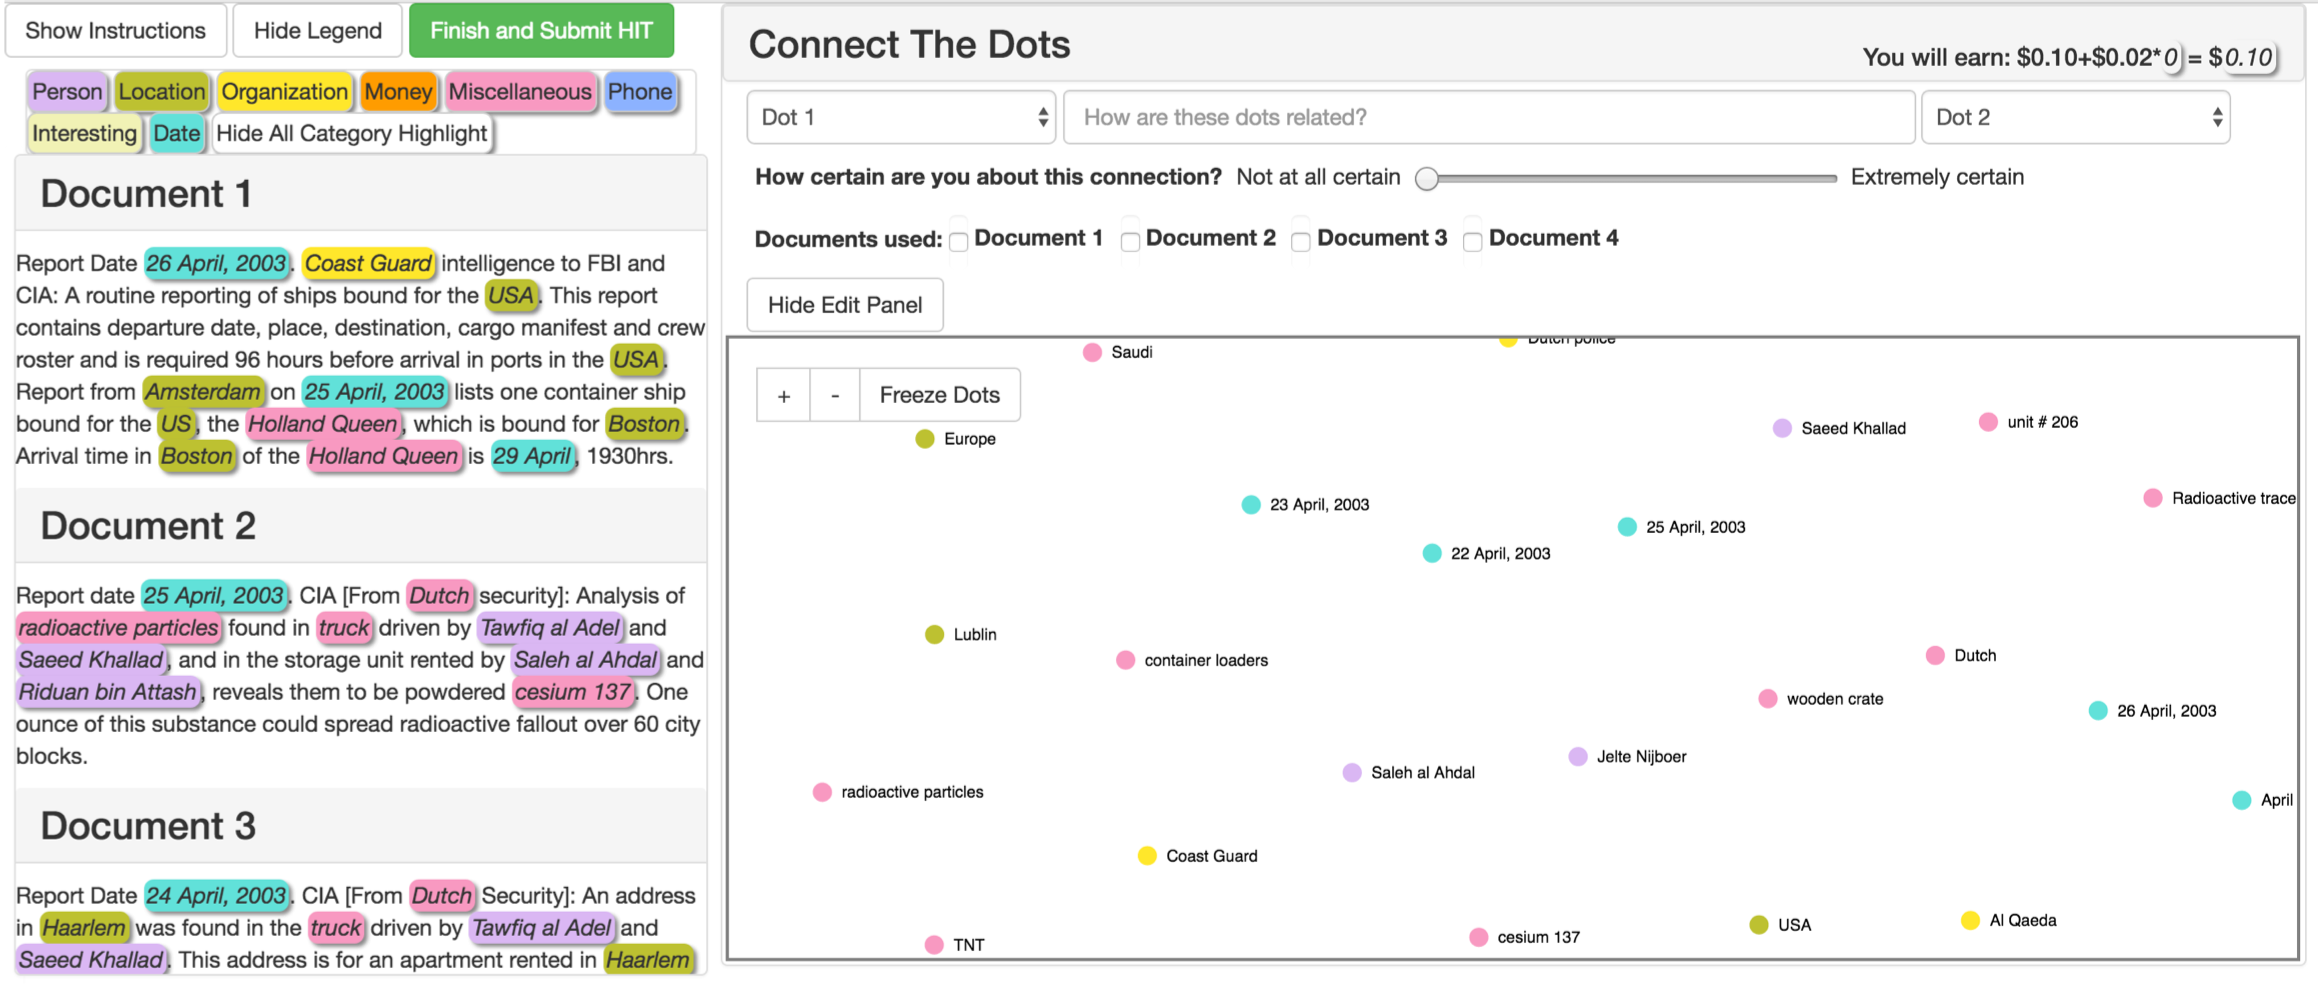
\includegraphics[width=\textwidth]{Hit}
 \caption{The Connect the Dots web application interface}
 \label{fig:hit}
\end{figure*}

说明一下系统是用了机器学习的东西的,为了保证其他交互和StartSPIRE的一致.
CrowdSPIRE (Crowd-powered Spatial Paradigm for Information Retrieval and Exploration) is a visual analytics tool prototype that implements crowd-powered semantic interaction technique: like ForceSPIRE, a semantic interaction visual analytics tool prototype for exploring unstructured text documents.
CrowdSPIRE and ForceSPIRE share a flexible spatial workspace (driven by a modified force-directed layout and several semantic interactions.
However, with different models on the background to help calculate the layouts of documents.
Instead of using machine learning models, CrowdSPIRE use human computation to help calculate the distance between documents and update the layout of workspace.

Right now, CrowdSPIRE integrate the "Connect the dots" tasks, which let crowds labels related entities in documents in a context slice and helps crowd workers with the micro-task of creating and labeling connections between entities extracted from the text.
Through related entities in each document, we could calculate their TF-IDF similarity. When doing overlapping two documents.
This system extends upon previous work to integrate relevance-based retrieval and layout models, provides richer visual encodings, and adds to the semantic interactions leveraged.

StarSPIRE dynamically adjusts how many data points are displayed by using heuristic-based relevance metrics.

Difference from basic pipeline.
% Crowd-sourcing part
% Document overlapping part.

%%%%%%%%%%%%%%%%%%%%%%%%%%%%%%%%%%%%%%%%%%%%%
%	Visual Encoding
\subsection{Visual Encodings}
Within the spatial workspace, document nodes are visually encoded to relate their relevance to the user’s high dimensional understanding of the data [Figure 5].
Node size and saturation are encoded to reflect how closely a document matches the entities the user has deemed important.
Node size and saturation are calculated by summing all of the entity weights in a document, ranking these values, and sorting them into quartiles.
Quartiles were chosen instead of absolute
ranking to optimize the node drawing process, minimizing the number of calculations and changes required with each user interaction.
This was done to promote a quick interaction-feedback loop.
These encodings give the illusion of a third dimension in the workspace where more important documents are in the foreground while less important documents fade into the background.
However, unlike a true three-dimensional layout, document nodes cannot overlap each other, preventing occlusion.
Additionally, StarSPIRE provides visual cues for navigating the workspace.
Node color is used to indicate search term matches.
Instead of showing all links between all documents, StarSPIRE restricts the edges shown to those connected to the selected node.
Entities shared between documents are labelled on the edge, but are restricted to the top four entities, determined by their importance weights.
All nodes are labelled with their document’s titles in order to allow for easier navigation in the space and to allow users to track a specific node’ s movement throughout the space.
Each node’ s outline color is used to denote its read or unread status in order to allow analysts to see which documents they have read and closed.

Within each document, search terms are identified and the text color is changed to allow the terms to stand out for easier identification.
These encodings were identified and/or adjusted through an informal usability requirements analysis of StarSPIRE.

%%%%%%%%%%%%%%%%%%%%%%%%%%%%%%%%%%%%%%%%%%%%%
%	Crowd-powered Document Overlapping
\subsection{Crowd-powered Document Overlapping}
CrowdSPIRE implement all the interactions on ForceSPIRE, users could explore the whole datasets based on document movement, text highlighting, pining document, annotation sticky note, open document, minimize document and overlapping documents. However, to make the system simple and easy to evaluate, we only combine document overlapping interaction with crowdsourcing tasks.

To evaluate the crowd-powered semantic interaction model, we only combined the document overlapping interaction with crowdsourcing tasks.
At first, we have the distance between documents based on algorithms models.

We two or more documents overlapped each other, the semantic interaction will trigger the task allocation stregory design a connect the dots crowdsourcing, based on overlapped documents.

We define D as the set of overlapped documents, for each
To carry out the 'connect the dots' task that help synthesis the overlapped documents:
The task allocation strategy procedure that automatically assign current overlapping interactions to task:\newline
(1) Pick m documents d1, dj from D (i != j), for all the di, dj. \newline
(2) Generate a Hit to MTurk that show m documents:
(2)	Show di, dj to k workers on a visualization view sub-task, which requires workers connect the related entities if they are related. \newline
(3) For each link, the worker should input the certain, and how are these dots related. Document used to make this connection \newline

For example, if three documents d1, and d2 and d3 are overlapped to each other, one of the micro-tasks is on Figure 1: {d1, d2}, {d1, d3} ... will be formed to give tasks to differnet.

based two documents, the connect the dots will publish an Hit on MTurk

%	Integrate 'Connect the Dots' into Workspace
%%%%%%%%%%%%%%%%%%%%%%%%%%%%%%%%%%%%%%%%%%%%%
% Integrate
\subsection{Integrate "Connect the Dots" into Workspace}
To make full use of the 'Connect the Dots' tasks as a real time services, we prototype the task, before the overlapping interactions.
For example, instead of design the hit, after the semantic interaction, we pre-assigned the task, and store outputs to the database, when the overlapping interaction be implements, we retreave this context, as it is.
The related nodes could also be mapped to distances. based on
BAsed on algorithms. Aslo, mapping the distance functions based on related entities.
Pre-store current storage to mimic the real time crowdsourcing.

%%%%%%%%%%%%%%%%%%%%%%%%%%%%%%%%%%%%%%%%%%%%%
% Case Study
%%%%%%%%%%%%%%%%%%%%%%%%%%%%%%%%%%%%%%%%%%%%%

%%%%%%%%%%%%%%%%%%%%%%%%%%%%%%%%%%%%%%%%%%%%%
% Evaluation
%%%%%%%%%%%%%%%%%%%%%%%%%%%%%%%%%%%%%%%%%%%%%
\section{USAGE SCENARIO}


In this section, we will demonstrate how CrowdSPIRE helps an analyst to make sense of complex dataset.
We use The sign of the Crescent dataset[ref] which contains 41 fictional intelligence reports regarding a coordinated terrorist plot in three US cities.
We will evaluate the effectiveness of CrowdSPIRE, we make a comparison of crowd-powered visual analytics (CrowdSPIRE) and algorithm-only based visual analytics (ForceSPIRE).
Also, to test that the crowdsourcing tasks outputs correctness that we compare the layout of documents based on crowdsourcing with the gold standard solution/and the most correct layouts we get when users make sense of documents.
\begin{figure*}
 \centering
  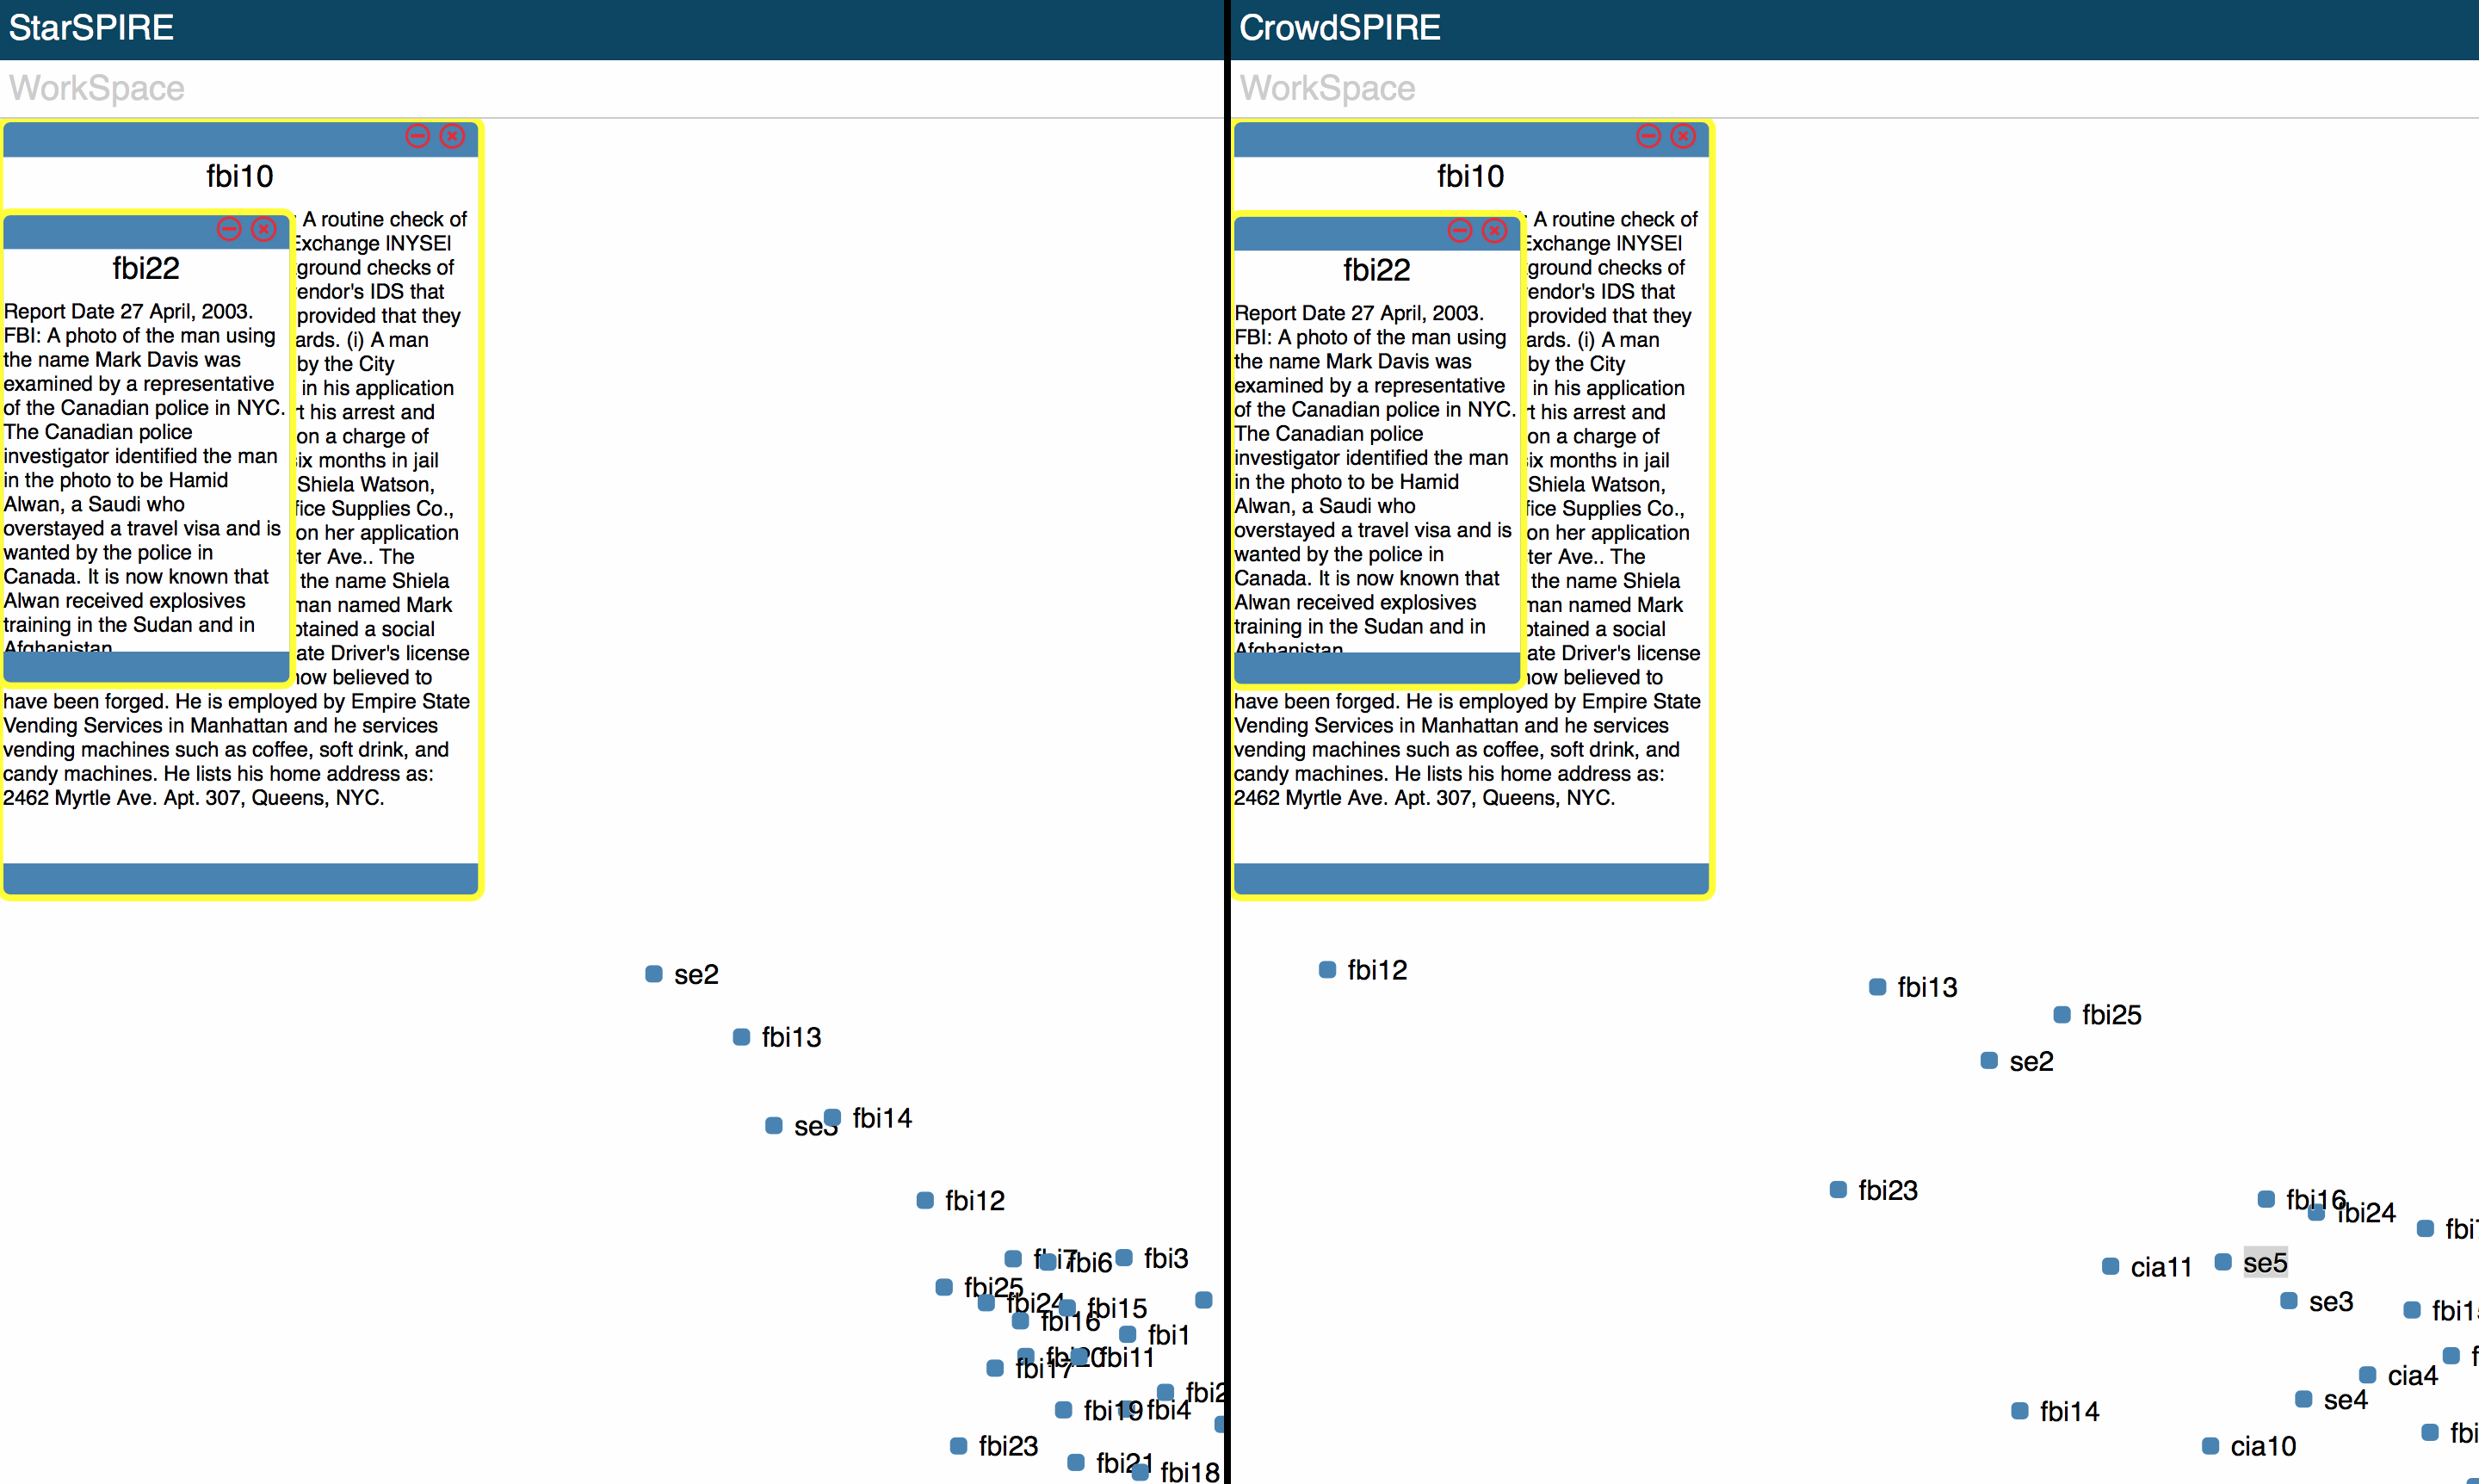
\includegraphics[width=\textwidth]{Case}
 \caption{A process of finding a major threat plot with key steps. (1): Based on A. Ramazi, finding that there are two similar bundles and two cells. (2): One name and two bundles are highlighted when hovering the mouse over B. Dhaliwal. (3): Three names and three bundles are highlighted when exploring F. Goba. (4) Referring to the four connected groups of useful entities for hypothesis generation.}
 \label{fig:case}
\end{figure*}

In this section, we walk through a text analytics scenario to demonstrate the how crowdsourcing supports
Comparison of crowd-enhanced version (CrowdSPIRE) with algorithm-only version(ForceSPIRE).

We prototype a web-version ForceSPIRE at the same version.
The different between ForceSPIRE and CrowdSPIRE is that when overlapping documents together:
ForceSPIRE will trigger the underlying machine learning alorithm to help calculatet the distance between documents.
CrowdSPIRE will trigger the crowd micro-tasks allcation alorithm to assign "Connect the Dots" micro-tasks, and then use the output to calculate the document distance.

So if we let the a user explore the doucments through this two documents, with the same interaction except overlapping documents, they will get similar layout.
Through the layout of overlapping documents interaction, we could analyse current layout that could help user make sense of documents.

For example, if we drag document together, the different layout on two techniques could help use analyse the effectiveness of CrowdSPIRE.

To demonstrate StarSPIRE’s functionality, we used the VAST 2007 Challenge Dataset (“Blue Iguanodon”) [17].
Because StarSPIRE is currently designed to operate on unstructured text documents only, we omitted all images and spreadsheets from the dataset, resulting in approximately 1,500 text files.
Blog entries that were included in the data were converted into text files, one for each blog entry.
Preliminary entity extraction was done on the dataset.
The challenge task is an open-ended sensemaking task to investigate “unexpected activities concerning wildlife law enforcement, endangered species issues, and ecoterrorism” [17].
We present the following usage scenario to demonstrate how StarSPIRE can leverage the MSI technique.
The user began with a search for “chinchilla.” This was unsurprising, because the dataset contained a directory titled “Chinchillas.”
She read through several documents, arranging them in the display based on document similarity.
The user then began highlighting information regarding chinchillas, which branched into additional endangered species.
This loosely structured analysis continued until the user read a document concerning a musical artist owning an extremely large number of exotic animals whose actions did not seem to match his words regarding animal conservation.
The analyst denoted this as suspicious and began investigating it further.
 This investigation was driven through highlighting the artist’s name and the name of his animal sanctuary, which imported many documents onto the display, some of which had a large node size.
  The analyst opened the largest new nodes first.
[Figure 8] shows the evolution of the user’s spatial organization schemas through the sensemaking task.
Clusters of documents were moved around the screen and a mixture of visual encodings and document proximity motivated the choice of documents to investigate next.
Furthermore, it can be seen that the user initially executed two searches to obtain some initial documents, but then opted for other multi-scale semantic interaction techniques to obtain new documents (e.g. highlighting, linking documents – denoted by the purple bars, and annotating documents).
Document annotations were used to record hypotheses and insights (e.g. “r’Bert is r’Bear?” and “r’Bear might have monkeypox”).
In the later stages of analysis, searches were used primarily to label the space, serving as reminders of which documents concerns which persons or topics.
However, they were also used to ensure that important information or documents had not been overlooked.

Once the user identified suspicious activity regarding a large exotic animal reservation, it became apparent that many documents were interconnected via several subplots.
As her understanding of the dataset evolved, so did her spatial representation.
For example, two documents that were initially considered “not quite relevant, but interesting enough to not minimize” concerning an outbreak of a disease were initially placed in the upper right hand corner of the display.
After realizing that the owner of the large exotic animal sanctuary had contracted the same disease, she moved the two documents down next to the exotic animal sanctuary documents.
Highlights, document annotations, and document linking were primarily used to obtain new documents in the workspace.
Searches were executed to check for additional information on important persons, but also used to label the spatial workspace.
After approximately ninety minutes of analyzing the data, the user concluded that she had a sufficient understanding of the plot and subplots in the data.
The user’s results were compared with the known ground truth solution.
The user correctly identified four out of five subplots in the data.
The use added 145 documents to the workspace, which is 10% of the actual dataset.
47 documents were opened and 33 remained open at the conclusion of the sensemaking session.
The user made eight searches, four document annotations, and 21 highlights.
45 documents were added through searches, whereas the remaining 100 documents were added through other multi-scale semantic interactions (e.g. highlight, annotate, document proximity).
Out of 26 documents relevant to the final solution, the user had added 18 of them to the workspace.
Six of these 18 documents were added through an explicit search, while twelve were added through implicit multi-scale semantic interactions.
13% (6/45) of documents added through explicit searches were relevant to the solution, and 12% (12/100) of documents added through implicit searches were relevant to the solution.
Therefore, the documents that originated from multi-scale semantic interactions were similar in quality to those that originated from explicit searches from the user.
Out of approximately 1,500 documents, 47 were read.
Thus, the analyst was able to construct 80% (four out of five subplots) of the solution while only reading 3.13% of the documents in the dataset.
While the results of this usage scenario appear promising, further work is required to evaluate the performance of MSI techniques as compared to existing SI techniques.



We get the conclusion that:

1. If Crowds could help remove noises from when sensemaking, to find most imports trifiles/dots.
2. If Crowds could help group close dots together.
3. If Crowds could provides external knowledge that not list on documents.

1. Crowds could help remove the noise, that are irrelebant details, dots, or trifles, even they are closed related to important documents.
three assignments contained little or no "noise" in the form of irrelevant details, dots, or trifles. I
embedded in an array of irrelevant dots that exist in intelligence reports that will lead the students nowhere as far as the hypothesis that is suggested by the relevant dots.

2. Crowds could be helpful for simultaneous and coordinated terrorist activities involving three actions planned for
3. Provides knowledge that not included in documents. most important element of imaginative and productive intelligence analysis in real life.

have included a variety of irrelevant or distracter items.
In short, skillful and thorough intelligence analysis requires that you carefully find out about what some dot or trifle is telling you.
Such knowledge is not always, perhaps only rarely, revealed in the reports in which these dots or trifles are given to you.
different persons will generate different hypotheses from the same body of evidence.

produces different insight?
better insight???
compare to Gold Standard Solution
beyond simple keywords, semantics similarities
compare to previous user study cluster results?

How the assigned tasks is good to current tasks.
Comparison of crowd-enhanced version with algorithm-only version
produces different insight?
better insight???
compare to Gold Standard Solution
beyond simple keywords, semantics similarities
compare to previous user study cluster results?
Finally we find that .

%%%%%%%%%%%%%%%%%%%%%%%%%%%%%%%%%%%%%%%%%%%%%
%	Conclusion
%%%%%%%%%%%%%%%%%%%%%%%%%%%%%%%%%%%%%%%%%%%%%
\section{Conclusion and Future Work}

We present crowd-powered semantic interaction model, a visual analytics model, which help analysts make sense of documents quickly through the help of crowdsourcing.
In this model, we use semantic interaction to enable users to steer the crowdsourcing assginement implicitly instead of require users of domain knowledge fo crowdsourcing.
In addition, we provide several different ways to help combine the crowd outputs back into the workspace(visual interface)) appropirately based on current visualization layout.
% tells more about crowd-powered semantic interactions.
Moreover, this model also takes the combination of human computation and automatic computation.
That automatic computation methods, like, machine learning could be used to find more related data that can be used in mirco-tasks.
The outputs from crowds, could help update the layout of workspace directly, or undirectly through providing more knowledge for automatic computation methods.
For example, more semantic links between documents or entities could help improve the correctness of machine learnning algorithms, when doing clustering.
With a usage scenario, we demonstrate how crowdsourcing can potentially support an analyst to explore complex sensemaking tasks.
However, there are still three challenges that need further explorations.
Current version of CrowdSPIRE only contains the basic needed components of: Visualization, Anlytic model and Crowd part "Connect the Dots".
More works needed to be done on this parts:


C1: Find the most appropriate crowdsourcing tasks for current visual analytic system.
In CrowdSPIRE, we combine the visual analytic system with machine learning algorithms, and basic crowdsourcing tasks "Connect the Dots".
The connection between semantic interactions with "Connect the Dots" shows us crodsourcing could provides help that machines are inadequacy to do right now.
However, there are lots of crowdsourcing tasks that we could do for each interaction, which we must perfom lots of experiements to find the best solution.

C2: Ways to integrate crowdsourcing output into workspace.
Current ways of integrate crowdsourcing into workspace, is pre-perfoming all the needed micro-tasks, and store the outputs permanently.
When some interactions intrigger some specific micro-tasks, we just search for related micro-tasks results directly from database, instead of carry out a real-time HIT.
Several other ways of carry out tasks should be considered: how to carry out real-time hits instead of the prostored results.
More integrating ways needed to be explored, to find the best stretegy to comnbine crowdsourcing and visual analytics.


C3: Comparision between crowdsourcing and machine learning algorithms.
CrowdSPIRE give a simple demo on how could we combine crowdsourcing together with machine learning algorithms to help analysts' sensemaking.
However, we must doing more research on finding which part is good at what kinds of tasks.
So the semantic interaction could decide assign what kind of tasks to crowds and other tasks to machine learning algorithms.


%\bibliographystyle{abbrv}
\bibliographystyle{abbrv-doi}
%\bibliographystyle{abbrv-doi-narrow}
%\bibliographystyle{abbrv-doi-hyperref}
%\bibliographystyle{abbrv-doi-hyperref-narrow}

\bibliography{template}
\end{document}

